\section{Experiments}
\label{sec:exp}
\begin{figure*}[!htb]
    \centering
    \vspace{-5pt}
    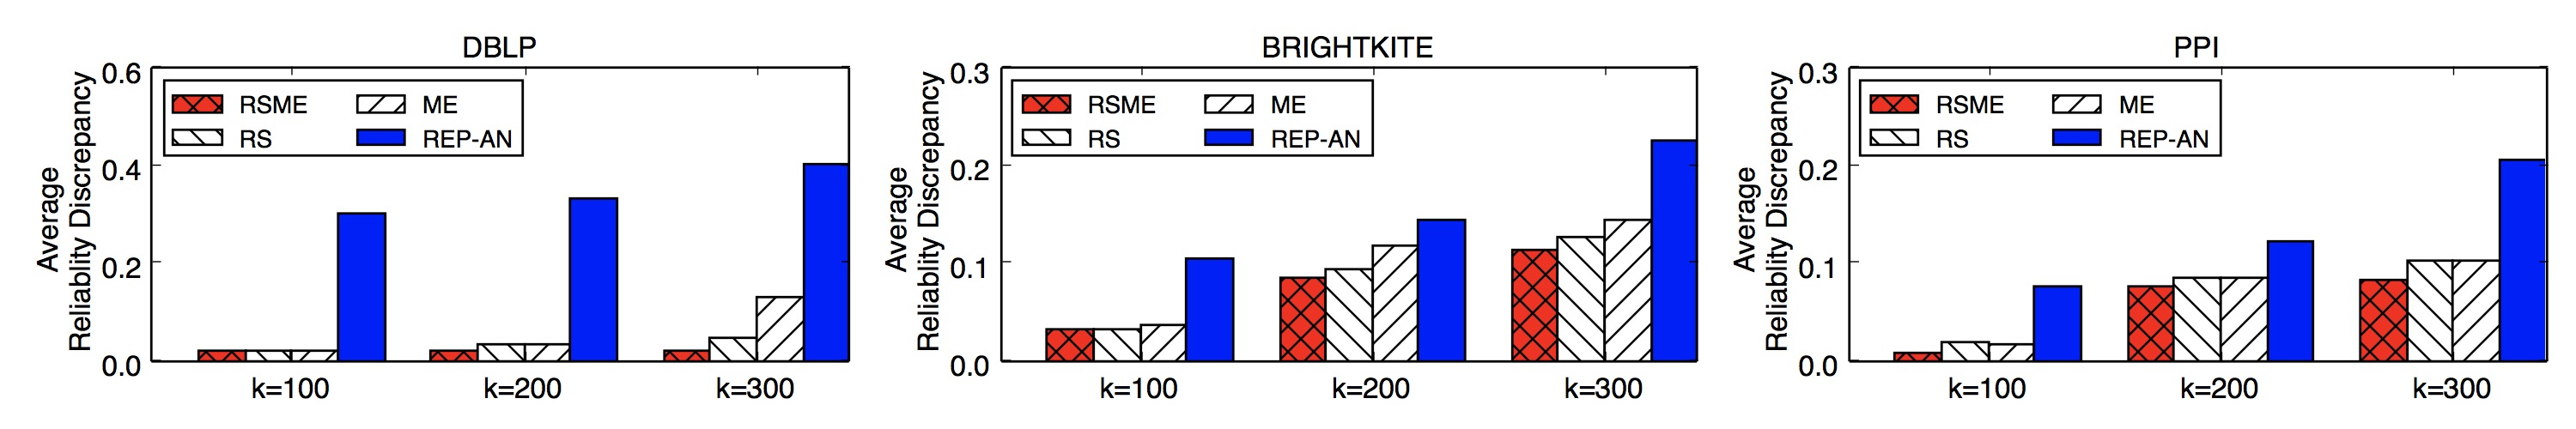
\includegraphics[width=\linewidth]{exp/exp_rel.jpg}
    \caption{Comparison of anonymization methods in terms of their ability to preserve Reliability.}
    \label{fig:ex_rel}
    \vspace{-5pt}
\end{figure*}
\begin{figure*}[!htb]
    \vspace{-5pt}
    \centering
    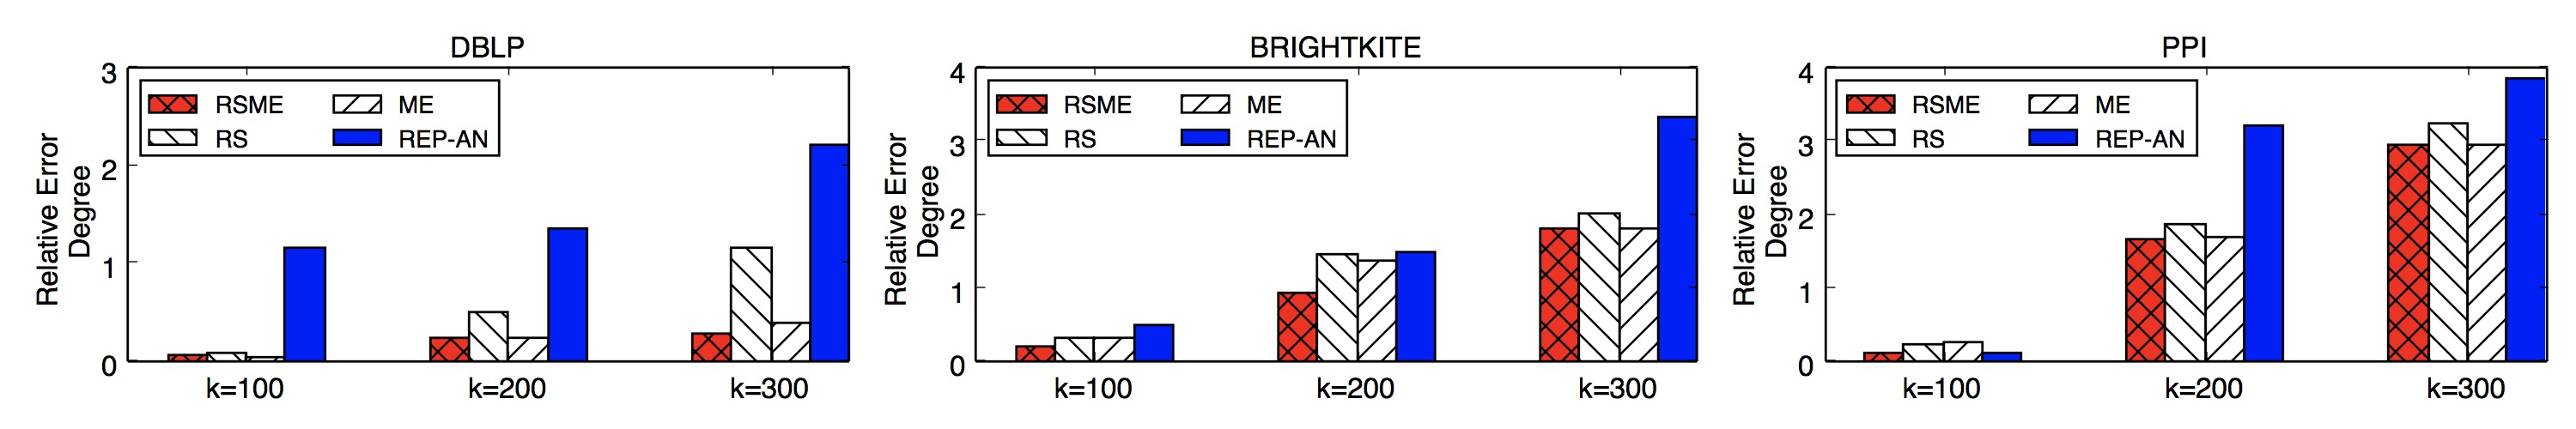
\includegraphics[width=\linewidth]{exp/exp_degree.jpg}
    \caption{Comparison of anonymization methods in terms of their ability to preserve Average Node Degree.}
    \label{fig:ex_degree}
    \vspace{-5pt}
\end{figure*}

In this section, we evaluate how well Chameleon and its variants preserve a \emph{uncertain} graph's structural statistics by comparing its anonymized \emph{uncertain} graphs against the original one in terms of graph metrics. The evaluated methods are Chameleon (RSME), RS (Reliability Sensitive), ME (Maximization Entropy) and Rep-An (Representative Anonymization).
Strong structural similarity (small error) in these results would establish the utility of these anonymized graphs in real research analysis and experiments. 

\subsection{Evaluation Methodology}

%-----------------------------------
%  Compared methods
\begin{table}[t]
    \small
    \caption{Summary of compared methods. }
    % \vspace{-1em}
    \newcommand{\tabincell}[2]{\begin{tabular}{@{}#1@{}}#2\end{tabular}}
    \centering
    \scalebox{0.95}{
    \begin{tabular} {|l|c c c|c|}
    \hline 
    Method & \tabincell{c}{Uncertainty \\-aware }  &  \tabincell{c}{Reliability \\-oriented} & \tabincell{c}{Anonymity \\-oriented} & Source \\
    \hline   \noalign{\vskip 1.5mm} \hline
    Rep-An  & -- & --& \checkmark & \cite{Parchas_Gullo_Papadias_Bonchi_2014}+\cite{Boldi_Injecting_2012} \\
    \hline 
    RSME & \checkmark & \checkmark & \checkmark & This work \\
    \hline 
    ME & \checkmark  & -- & \checkmark &  This work   \\
    \hline 
    RS & \checkmark  &\checkmark & --  &   This work  \\
    \hline 

   \end{tabular}
   }
   \vspace{-10pt}
    \label{tab:methods}
\end{table}
%-----------------------------------

\textbf{Metrics.}~~Besides reliability, our evaluation includes three classes of graph metrics. One group includes degree-based metrics such as Average Node Degree, Degree Distribution, Maximal Degree. These are basic topological metrics capture how degree distributed among nodes. The second group includes node separation metrics such as Average Distance, Graph Diameter. They are used to quantifying the inter-connectivity of the graph. The third group metrics include Clustering Coefficient which measures how close neighbors of a node are to forming cliques. 

\textbf{Computation.}~~Since there does not exist the closed formula for graph metrics expect Average Node Degree, the results are approximated by Monte Carlo sampling. Specifically, we create a number of random instances of an uncertain graph, and we compute the expected value of each metric using the average of the sampled graphs. Here, we use 1,000 samples since it has been shown that $1000$ usually suffices to achieve accuracy converge~\cite{Potamias_K_2010,Jin_Distance_2011}. In particular, we use Approximate Neighborhood Function (ANF) \cite{Boldi_Rosa_Vigna_2011}, to approximate shortest path-based statistics. For each metric, we report the ratio of absolute difference against the original one. 

\textbf{Parameter Setting.}~~We generate anonymized \emph{uncertain} graphs for $k \in [100,300]$ and compare the graph metrics of the resulting \emph{uncertain} graphs against those original graphs. We limit ourselves to obfuscation levels, $k \in [100,300]$ following reasons. 
First, we aim to explore the case the desired privacy level requires a small amount of noise ($k=100$). This way, we can quantify the utility loss difference introduced by Chameleon against Rep-An method. Second, it naturally requires a high level of noise to provide strong levels of privacy guarantees. We want to explore the sensitivity of different variants. Unfortunately, very large values of $k$ require large noise, thus producing anonymized graphs that are extremely different from the original ($k=300$). 


\subsection{Results}
\textbf{Reliability.}~~Figure~\ref{fig:ex_rel} compares the average reliability discrepancies. The smaller discrepancy, the better the reliability preserving. In all cases, the Chameleon (RSME) performs best, followed by its variants (RS and ME).

For each of the DBLP, BRIGHTKITE and PPI graphs, the reliability of Chameleon ($k=100$) output graphs are very close the ones of the original graphs. When we increase the strength of the privacy guarantees, i.e., larger $k$ values of $200$ and $300$, the error of average reliability progressively increases. Our experiments show the errors introduced by Chameleon (RSME) only increase slowly as $k$ value increases. Note that RS strategy (less perturbation over ``bridge"-like edges) does provide the beneficial impact on the reliability preserving (as witnessed by the smaller error introduced by RSME v.s. ME).

\textbf{Degree-based Metrics.}~~For brevity, we only report results for  Average Node Degree, as representative of degree-based metrics in Figure~\ref{fig:ex_degree}. For each of the DBLP, BRIGHTKITE and PPI graphs, the average node degrees of Chameleon ($k=100$) output graphs are very close the ones of the original graphs. When we increase the strength of the privacy guarantees, i.e., larger $k$ values of $200$ and $300$, the error of average degree slowly increases. For example, DBLP graph shows a small deviation even for $k=300$. The worst-case average degree deviation introduced by the RSME method is still within 15\% of the original. 

On the other hand, BRIGHTKITE and PPI show slightly different behaviors. For large $k$ values, i.e., $k=200$ and $k=300$, the largest error is over 300\% from the original values. The root of large errors is the existence of heavy-tailed degree distribution (over 4\%) in these two graphs which requires larger amount of noise. 

Among Chameleon variants, RS is clearly outperformed by ME and RSME methods in all datasets. For example.  average degree deviation introduced by RS (1.16) is much larger ones of other variants (0.39 and 0.27) in DBLP dataset. This is encouraging because we can eliminate the bulk of the error by fine-grained control of edge probability alteration.   

\begin{figure*}[!tb]
    \centering
    \vspace{-5pt}
    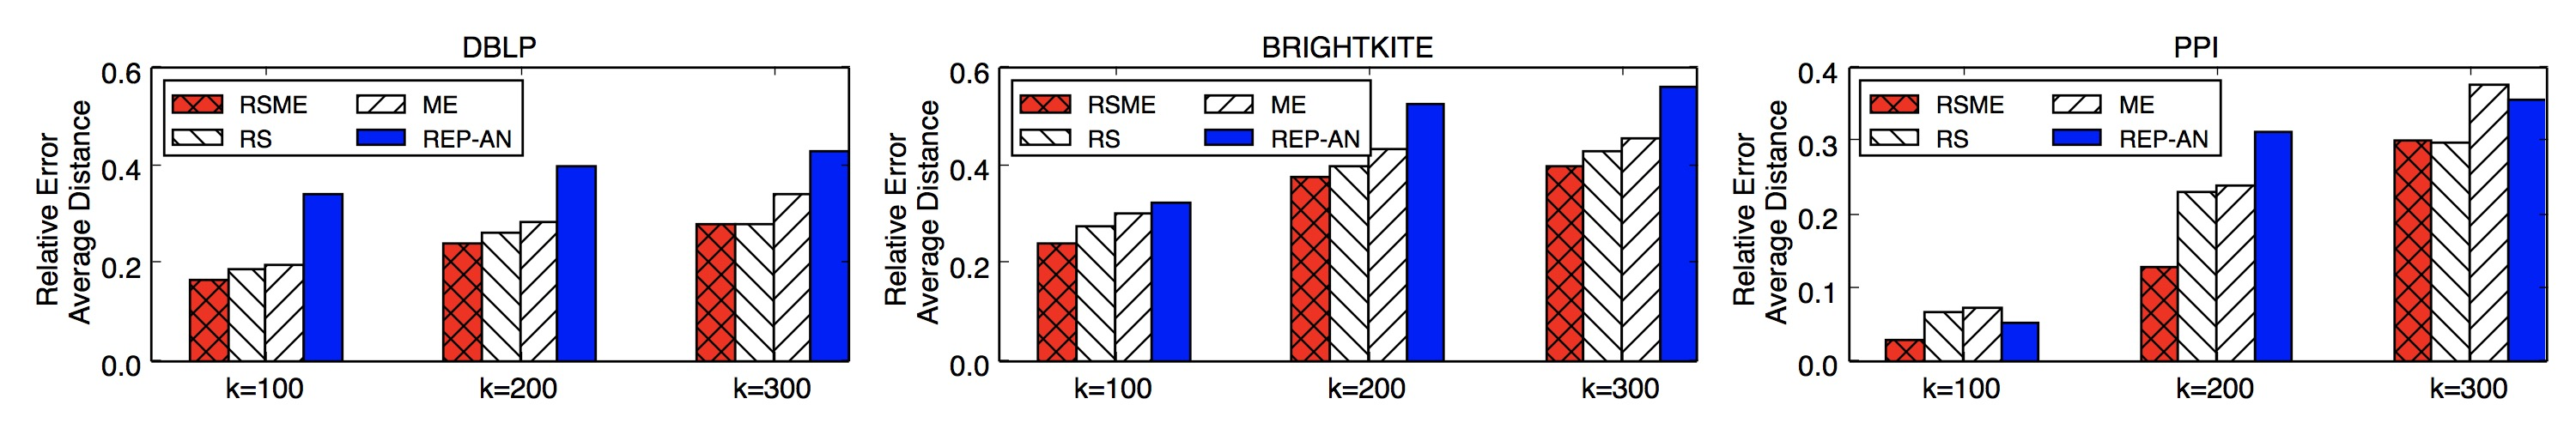
\includegraphics[width=\linewidth]{exp/exp_apd.jpg}
    \caption{Comparison of anonymization methods in terms of their ability to preserve Average Distance.}
    \label{fig:ex_apd}
    \vspace{-5pt}
\end{figure*}

\begin{figure*}[!tb]
    \centering
    \vspace{-5pt}
    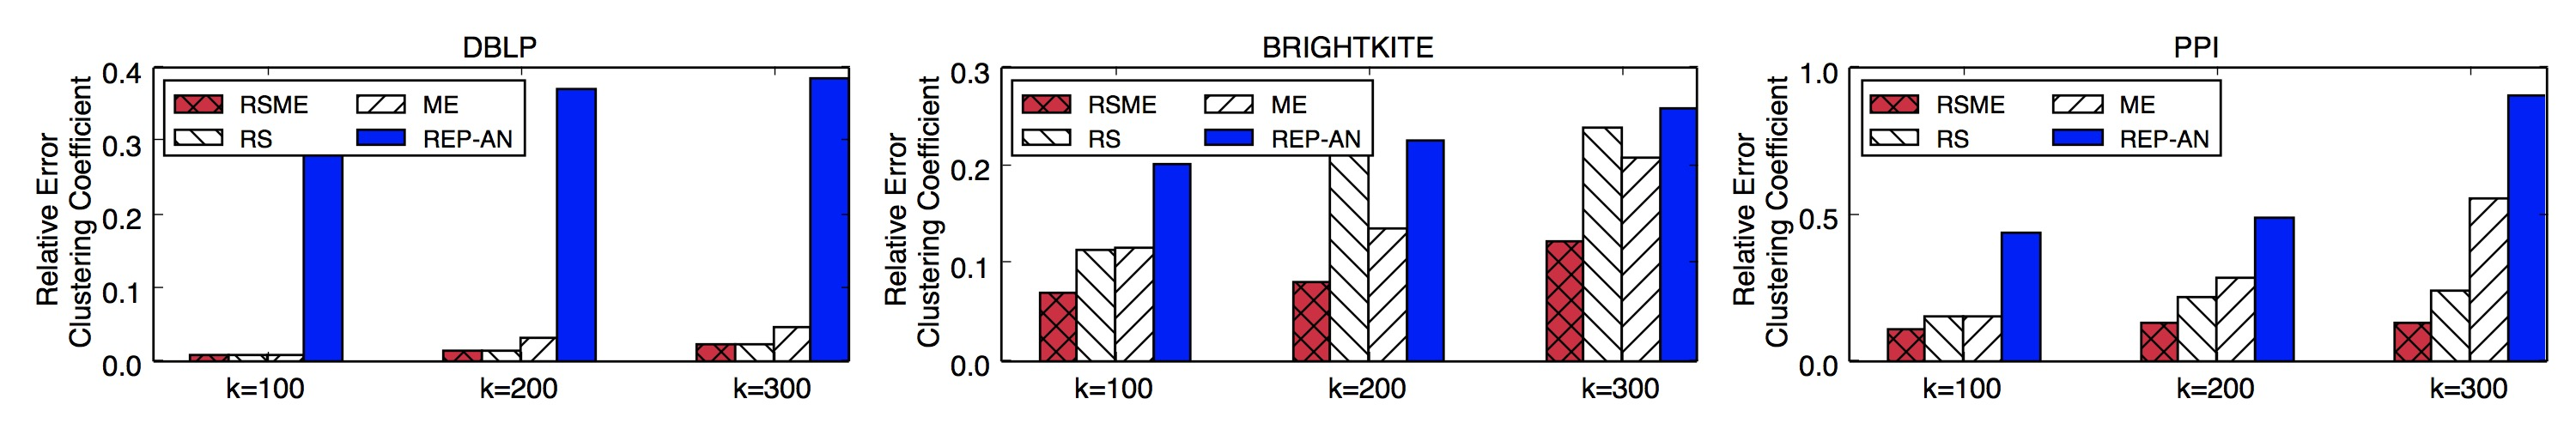
\includegraphics[width=\linewidth]{exp/exp_cc.jpg}
    \caption{Comparison of anonymization methods in terms of their ability to preserve Clustering Coefficient.}
    \vspace{-5pt}
    \label{fig:ex_cc}
\end{figure*}
% \vspace{-5pt}

\textbf{Node Separation Metrics.}~~For brevity, we report only the Average Distance as a representative of the node separation metrics. Figure~\ref{fig:ex_apd} shows the Average Distance (AD) values computed on DBLP, BRIGHTKITE, and PPI graphs compared to the AD values on their anonymized graphs.  

\textbf{Clustering Coefficient}~~In comparison, the error introduced by strengthening privacy (i.e., increasing $k$) is relatively small. As with previous experiments, the BRIGHTKITE graph shows a little different behavior. In this case, all of Chameleon output graphs do a good job of preserving Clustering Coefficient of the original graphs (well below 15\%). It confirms the close relationship between reliability and clustering coefficient.


\textbf{Summary.}~~Our experimental evaluation on real-world datasets confirms the initial and driving intuition: the {\SysNameNS} approach which explicitly incorporates edge uncertainty and the possible world semantic in the anonymization process outperforms the benchmark solution Rep-An significantly regarding the uncertain graph utility preservation. The {\SysNameNS} introduces limited impact as a result of adding noise to guarantee privacy.  

Another take-home message is: by using fine-grained and uncertainty-aware perturbation strategies such as reliability sensitive edge selection (RS) and max entropy based edge prob alteration (ME), one can achieve the same desired level of obfuscation with the smaller change on the uncertain graph thus maintaining higher data utility. 




